\documentclass[12pt,letterpaper,noanswers]{exam}
\usepackage[usenames,dvipsnames,svgnames,table]{xcolor}
\usepackage[margin=0.9in]{geometry}
\renewcommand{\familydefault}{\sfdefault}
\usepackage{multicol}
\pagestyle{head}
\header{AM 111 Class 03}{}{Compressing data via a model, p.\thepage}
\runningheadrule
\headrule
\usepackage{siunitx}
\usepackage{enumitem}
\usepackage{graphicx} % more modern
\usepackage{amsmath} 
\usepackage{amssymb} 
\usepackage{hyperref}

\usepackage[most]{tcolorbox}
\usepackage{listings}

\definecolor{white}{rgb}{1,1,1}
\definecolor{mygreen}{rgb}{0,0.4,0}
\definecolor{light_gray}{rgb}{0.97,0.97,0.97}
\definecolor{mykey}{rgb}{0.117,0.403,0.713}

\tcbuselibrary{listings}
\newlength\inwd
\setlength\inwd{1.3cm}
% https://tex.stackexchange.com/questions/340700/ipython-notebook-input-and-output-cells-with-listings
\newcounter{ipythcntr}
\renewcommand{\theipythcntr}{\texttt{[\arabic{ipythcntr}]}}

\newtcblisting{pyin}[1][]{%
  sharp corners,
  enlarge left by=\inwd,
  width=\linewidth-\inwd,
  enhanced,
  boxrule=0pt,
  colback=light_gray,
  listing only,
  top=0pt,
  bottom=0pt,
  overlay={
    \node[
      anchor=north east,
      text width=\inwd,
      font=\footnotesize\ttfamily\color{mykey},
      inner ysep=2mm,
      inner xsep=0pt,
      outer sep=0pt
      ] 
      at (frame.north west)
      {\refstepcounter{ipythcntr}\label{#1}In \theipythcntr:};
  }
  listing engine=listing,
  listing options={
    aboveskip=1pt,
    belowskip=1pt,
    basicstyle=\footnotesize\ttfamily,
    language=Python,
    keywordstyle=\color{mykey},
    showstringspaces=false,
    stringstyle=\color{mygreen}
  },
}
\newtcblisting{pyprint}{
  sharp corners,
  enlarge left by=\inwd,
  width=\linewidth-\inwd,
  enhanced,
  boxrule=0pt,
  colback=white,
  listing only,
  top=0pt,
  bottom=0pt,
  overlay={
    \node[
      anchor=north east,
      text width=\inwd,
      font=\footnotesize\ttfamily\color{mykey},
      inner ysep=2mm,
      inner xsep=0pt,
      outer sep=0pt
      ] 
      at (frame.north west)
      {};
  }
  listing engine=listing,
  listing options={
      aboveskip=1pt,
      belowskip=1pt,
      basicstyle=\footnotesize\ttfamily,
      language=Python,
      keywordstyle=\color{mykey},
      showstringspaces=false,
      stringstyle=\color{mygreen}
    },
}
\newtcblisting{pyout}[1][\theipythcntr]{
  sharp corners,
  enlarge left by=\inwd,
  width=\linewidth-\inwd,
  enhanced,
  boxrule=0pt,
  colback=white,
  listing only,
  top=0pt,
  bottom=0pt,
  overlay={
    \node[
      anchor=north east,
      text width=\inwd,
      font=\footnotesize\ttfamily\color{mykey},
      inner ysep=2mm,
      inner xsep=0pt,
      outer sep=0pt
      ] 
      at (frame.north west)
      {\setcounter{ipythcntr}{\value{ipythcntr}}Out#1:};
  }
  listing engine=listing,
  listing options={
      aboveskip=1pt,
      belowskip=1pt,
      basicstyle=\footnotesize\ttfamily,
      language=Python,
      keywordstyle=\color{mykey},
      showstringspaces=false,
      stringstyle=\color{mygreen}
    },
}





\newcommand{\note}[1]{\textcolor{red}{#1}} % show notes in red
\renewcommand{\note}[1]{} % don't display notes

\begin{document}
 \pdfpageheight 11in 
  \pdfpagewidth 8.5in

\noindent 

\note{calendar:
\begin{enumerate}
    \item Tu binary subtraction, least sq intro PS01/2
    \item Th least sq PS02
    \item Tu lin alg PS02/3
    \item Th lin alg PS03
    \item Tu least sq PS03/4
    \item Th ?? PS04
    \item Tu root finding PS04/5
    \item Th root finding PS05 (early)
    \item Tu integration PS06
    \item Th quiz
    \item Tu interpolation PS06
    \item Th interpolation PS06
    \item Tu integration PS07
    \item Th Monte Carlo PS07
    \item Tu differentiation PS08
    \item Th differentiation PS08
    \item Tu diff eq
    \item Th application of diff eq
    \item Tu ODEs
    \item Th ODEs
    \item Tu neural nets
    \item Tu neural nets
    \item Th quiz
    \item Tu presentations
\end{enumerate}}

\note{
\begin{itemize}
    \item what is a floating point system
    \item example
    \item IDing info about a floating point system
    \item 
\end{itemize}
}
\setcounter{section}{-1}
\section{Preliminaries}
\begin{itemize}
\itemsep0pt
\item There will be a skill check in class during the next class.  The problem info is below.
\item Problem set 01 is due on Friday.
\item Labs and OH.
\end{itemize}

\hrule
\vspace{0.2cm}


\noindent\textbf{Big picture}
\begin{itemize}
    \itemsep0pt
\item Why do $3/2 - 1/2 - 1$ and $7/3 - 4/3 - 1$ give different results?
\begin{itemize}
    \itemsep0pt
    \item How is a real number represented in the computer?
    \item Where does error appear in that representation?
    \item How does that impact subtraction?
\end{itemize}
\item How do we compress information in a large dataset to only a few numbers?  
\begin{itemize}
    \item Once we have set up the problem mathematically, how do we find a solution?
    \item How do we measure the error in our solution method?
\end{itemize}
\end{itemize}

\vspace{0.2cm}
\hrule
\vspace{0.2cm}

\noindent \textbf{Skill check practice}

Given two binary numbers with the same number of bits after the radix point in their normalized representation, complete the following subtraction in binary:

$2.3 - 1.3$.

$2.3 = 1.001010_2\times 2^1 = 10.010100_2$

$1.3 = 1.010011_2 \times 2^0 = 1.010011_2$


\vspace{0.2cm}
\hrule
\vspace{0.2cm}

\noindent \textbf{Skill check solution}

You can use either

Direct subtraction:
\begin{align*}
&10.010100 \\
- &01.010011 \\
\cline{1-2}
&01.000001
\end{align*}

or ones complement:
\begin{align*}
&10.010100 \\
+ &00.101100 \\
\cline{1-2}
&11.000000
\end{align*}
Then add $1$ at the final digit and drop the leading $1$:
$1.000001$


\vspace{0.2cm}
\hrule
\vspace{0.2cm}


\section{Floating point in the computer}
\subsection{\texttt{float16}, \texttt{float32}, \texttt{float64}}

\begin{tabular}{ c | c | c | c| c}
name &bits & sign & exponent & mantissa\\
\hline
half &16 & 1 & 5 & 10 \\
single& 32 & 1 & 8 & 23 \\
double & 64 & 1 & 11 & 52 \\
longdouble& 80 & 1 & 15 & 64 \\
\end{tabular}



\subsection{Subtraction}

Binary subtraction can be done similarly to decimal subtraction.

A second algorithm is also sometimes used.

Example:
Find $1011.1 - 101.11$

Method 1:
\begin{align*}
&1011.10 \\
- & 0101.11 \\
\cline{1-2}
& 0101.11
\end{align*}

Check: $101.11 + 101.11 = 1011.10$

Method 2:

Compute $1011.10 + (111.11-101.11) + 0.01 - 1000.00$ instead (so add and subtract the same number).

This is a method called ones complement: $1011.10 + 010.00 + 0.01 - 1000.00 = 1101.10 + 0.01 - 1000.00 = 101.11$

\begin{enumerate}
    \item Compute $10.10100 - 1.10011$ using both methods.
\end{enumerate}

\section{Function fitting, Sauer \S 4.1}
\begin{itemize}
    \item In the reading for today you encountered the method of linear least squares, learning about the normal equations as a method of solution, and saw a reference to condition number / error in using that solution method.
    \item Today we will zoom out and talk about the broader problem of compressing data.
    \item We'll start by looking more generally at how to specify the problem of fitting a model to data, then will focus back in on linear least squares.
    \item As part of looking at the method, we will learn about the normal equations, about the condition number of a matrix, how these are sources of error, and about other solution methods.
\end{itemize}





\subsection{Representing and compressing data}

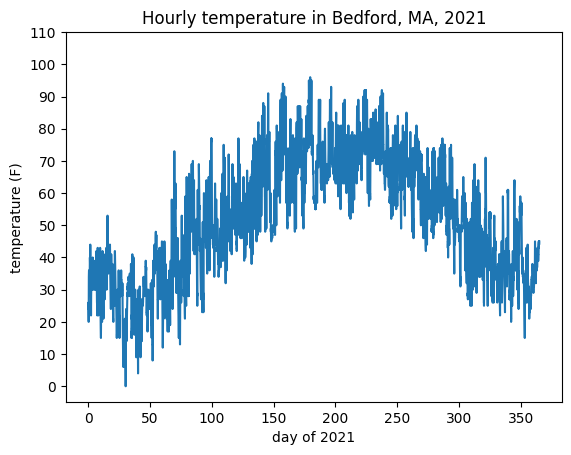
\includegraphics[width=0.45\linewidth]{img/C03weatherBedford.png}
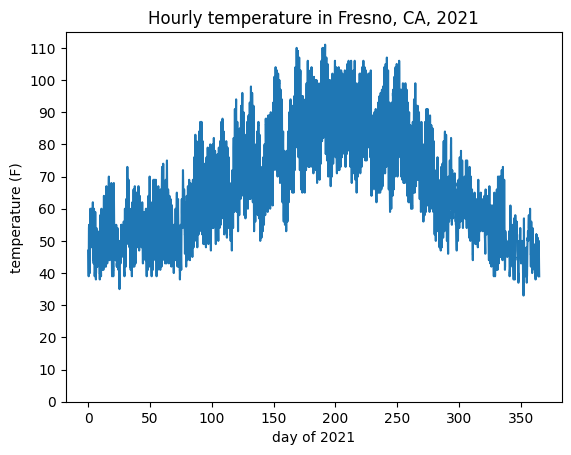
\includegraphics[width=0.45\linewidth]{img/C03weatherFresno.png}

NOAA NCEI data

\begin{enumerate}[resume]
\item If you had to summarize this data with a single number, how would you choose a number?  What number would you choose for the Bedford? What about the Fresno data?

% \emph{Have one member of your team use PollEverywhere \url{http://pollev.com/apmth111} to share your thoughts}

\item What if you could use two or three numbers (and a function of your choice)?  How would you summarize each dataset?
\end{enumerate}
\vspace{1cm}

\subsection{Lower dimensional representations}

Given a data set, our goal is to create a lower dimensional representation of the data.

When/how might such a representation be used?

Example: What is the typical temperature in Boston?

\begin{tcolorbox}
\begin{itemize}
\itemsep0pt
    \item approximate an ensemble (many temperature measurements) by a single number
    \item replace complicated behavior by a simple function (in this case a constant function)
    \item project a vector (the data) from a higher-dimensional space onto a lower-dimensional subspace
\end{itemize}
\end{tcolorbox}



\subsubsection{Modeling with a parametric function, Sauer \S 4.1.2}


\begin{tcolorbox}

\begin{itemize}
\itemsep0pt
    \item Let $\{(t_1, y_1), (t_2, y_2), ..., (t_m,y_m)\}$ be a set of data points.
    \item Choose a \textbf{model architecture}: identify a parameterized model, $y = f(t)$, that will be used to describe the data.  We have $y_i\approx f(t_i)$.

    For the method of linear least squares we will choose a model that is linear in its parameters.
    \item Choose a \textbf{measure of 'best'}: this is the cost function expressing the distance between $y_i$ and $f(t_i)$.
    
    Let $\mathbf{e} = (y_1-f(t_1),...y_m-f(t_m))$.  The vector $\mathbf{e}$ can be thought of as an error vector (error between the data and the fitting function).  The cost be computing using $\mathbf{e}$.

    For the method of linear least squares, the cost function a sum of squared errors.
\end{itemize}

\end{tcolorbox}

\begin{enumerate}[resume]
\item For each of the following functions $f(t)$, determine whether it is linear in $\mathbf{c}$, the vector of model parameters.  % If it is linear in $\mathbf{c}$, identify the basis functions $\varphi_k(x)$.
\begin{parts}
\item $f(t) = c_1 + c_2 t^2$
\item $f(t) = c_1 + c_2\sin(c_3 t)$
\item $f(t) = c_1e^t + c_2e^{2t}$
\item $f(t) = c_1 + c_2\sin t + c_3\cos t$
\item $f(t) = c_1e^t + c_2e^{c_3 t}$
\end{parts}

\item Model the data $\left\{(t_i,y_i)\right\}_{i=1}^3 = \left\{(0,1),(1,3),(2,0)\right\}$ with the function $f(t) = c_1$ where $c_1$ is a constant.
\begin{parts}
\item Write down $f(t_1)$, $f(t_2)$, $f(t_3)$, the approximations for $y_1, y_2, y_3$ produced by the model.
\item Construct the error vector, $\mathbf{e}$.
\item Use %$\Vert \mathbf{e}\Vert_2^2$ (the $2$-norm squared) 
the sum of the squares of the components of the error vector
as your cost function.  Construct the function and find $c$ to minimize it.

% \emph{Notice that $\Vert \mathbf{e}\Vert_2^2 = \mathbf{e}\cdot\mathbf{e}$}
% \item Use $\Vert \mathbf{e}\Vert_{\infty}$ as your cost function.  Find $c$ to minimize it.
% \item Use $\Vert \mathbf{e}\Vert_{1}$ as your cost function.  Assume $1\leq c\leq 3$ to simplify your $\vert \cdot\vert$ expressions.  Find $c$ (or a range of $c$) to minimize this.
% \item (extra) Show that for data $\left\{(x_i,y_i)\right\}_{i=1}^N$ the model $f(x) = c$, and the $2$-norm cost function, the value of $c$ that minimizes the cost function is $\left\langle
% y_i \right\rangle$, i.e. $\displaystyle c = \dfrac{1}{N}\sum\limits_{i=1}^N y_i$.
\end{parts}

% 

\end{enumerate}



\subsubsection{Cost functions: vector norms, Sauer \S 2.3, Greenbaum and Chartier \S 7.4.1}

For the method of linear least squares, we will focus on a cost function given by the sum of squared error (or the square root of the sum of squared error).

There are a few common cost functions, though, that are worth knowing about.

\begin{tcolorbox}
Three common/important cost functions:
\begin{itemize}
\itemsep0pt
    \item The \textbf{Euclidean norm} ($2$-norm): $\displaystyle\Vert\textbf{e}\Vert_2 = \sqrt{\sum\limits_{i=1}^m \vert e_i\vert^2}$
    
    For $\mathbf{e} = (x,y)$ this cost function is the familiar distance formula (for distance between $(x,y)$ and $(0,0)$).
    
    \item The $1$-norm: $\displaystyle\Vert\mathbf{e}\Vert_1 = \sum\limits_{i=1}^m \vert e_i\vert$
    
    \item The $\infty$-norm: $\displaystyle\Vert\mathbf{e}\Vert_{\infty} = \max\limits_{i=1...m} \vert e_i\vert$
\end{itemize}
\end{tcolorbox}

These cost functions are \textbf{norms}, or methods of measuring distance in a vector-space.

We can return to the constant model, using these other norms.

\begin{enumerate}[resume]
\item For your error vector, use the $\infty$-norm to find $c$.

\item Use the $1$-norm to find $c$.
\end{enumerate}



\end{document}